\section{Basic Assumptions}

The aim of this work is to propose a \gls{knx} prototype, applicable for environments with increased availability demands.
The prototype should be designed in a transparent way, utilizing a "plug and play" functionality to build a secure \gls{knx} network.
This means that a device outside of this network, unaware of
the secured \gls{knx} network, should be able to deliver through and receive messages from such a secured network without any prerequisites. 
Every device with one connection to an unsecured \gls{knx} network (called cleartext \gls{knx} line) and two distinct connections to a secured \gls{knx}
network (called secure lines, running the master daemon, will work
as a security gateway. Thus, the presence of at least 2 of these security gateways connected to each other by two secure lines will constitute a 
secured \gls{knx} area, bridging between areas with increased security demands, as shown in figure \ref{fig:secArea}.
\\
\\
The basic tasks of such security gateways consist of:
\begin{itemize}
 \item establishing keys with it's communication partners within the secured \gls{knx} network (the security gateways)
% \item maintaining some kind of synchronization token between all security gateways
 \item providing redundant communication lines, achieving improved availability by encrypting and authenticating all messages which are received on the unsecured line, and delivering them to the proper security gateways which act as
 border device for the given group address, using booth secure lines
 \item checking all messages which are received on the secured lines for integrity and authenticity, removing duplicates, unwrapping and delivering them to
 the unsecured area
\end{itemize}

\subsection{Security Related Architectural Overview}

As stated in chapter \ref{ch:knx}, 3 different possibilities for communication within a \gls{knx} network are possible: point to point, multicast and broadcast.
To introduce as little additional traffic into the network as possible, a sound concept for translating clear- to secure-\gls{knx} address (and vice versa) has to
be defined. While in principle it would be possible to use the communication modes in a transparent way (i.e., point-to-point in unsecured \gls{knx} translates
to point-to-point in secured \gls{knx}, and vice versa, and so on), this approach leads to some serious problems, rendering this solution impracticable:
due to the topology of \gls{knx}, it is impossible to know a priori the exact physical location of a device (i.e., its individual address). Additionally,
every device can be member of an arbitrary number of group addresses (bounded by the maximum number of group addresses), which also is not known in advance.
Group-membership is also subject to change and therefore complicates the situation. Finally, devices can leave or join the network at every moment by powering the
device up or down.
\\
Therefore, a device which receives a message on its unsecured \gls{knx} line, examining the destination address, simply does
not know which device(s), if any, will be the gateway(s) responsible for delivering this datagram one hop toward its final destination, regardless if the destination address
is a group- or an individual address.
\begin{figure}
    \centering
    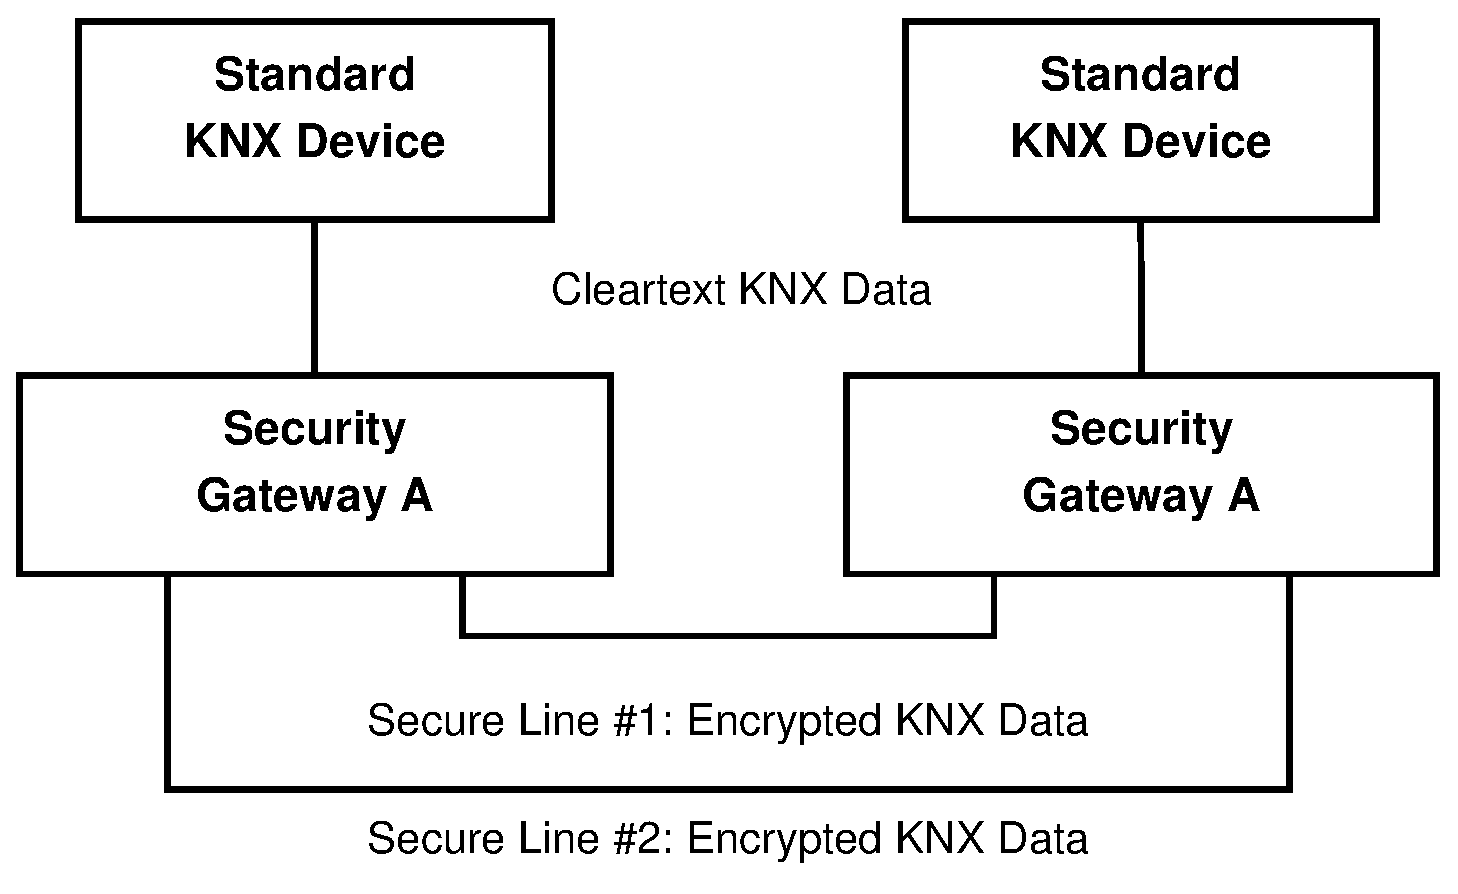
\includegraphics[width=1\textwidth]{figures/SecureArea.eps}
    \caption{Secure Area}
    \label{fig:secArea}
\end{figure}
\\
\\
A straightforward solution to this problem would be to wrap every datagram which enters the secured \gls{knx} network via a security gateway into a new, properly secured
broadcast datagram, and delivering this new package to the secured \gls{knx} network. Then, the package would be available to all other security gateways, which
will unwrap it and forward the resulting inner datagram to its unsecured \gls{knx} line. If the destination address (group or individual) of the actual payload
is assigned to a device connected
to the unsecured \gls{knx} network, the device holding this individual- or group-address will recognize it and the package will reach its destination. 
Otherwise it will simply be discarded.
\\
A serious constraint rising from this broadcast approach is that a single,
global network key must be used, because every security gateway must be able to decrypt and check every package which it receives on it's secured lines,
even if it does not serve as gateway to the wanted group address. 
The key of course can be renegotiated among the security gateways at every time, but this approach is considered
unsafe because an attacker can target \textit{any} of the security gateways constituting the secure network. An adversary breaking one single device gains
access to the network traffic of all devices. This could be achieved by physical access to any of the security gateways, for example by reading out the
memory of the device, and thus obtaining the globally used network key. This way, the network traffic can be decrypted by the adversary as long as no new
key is renegotiated. Another problem is that multi-party key negotiation is a costly task if a public-private key scheme
is to be used: as shown in figures \ref{fig:dh1} and \ref{fig:dh2}, a lot of messages have to be exchanged before actual an encryption can be done. 
\\
\\
To encounter this problems, different keys must be used, thus achieving pairwise end-to-end encryption between all devices. 
%This way it is also possible to achieve different security levels, depending on the function a 
%particular unsecured \gls{knx} device fulfills. It would be possible, for example, to distinguish between 'normal' gateways and 'hardened'
%gateways which are specially guarded against physical access, for example by applying physical intrusion detection. Thus,
%the risk of breaking the whole system is reduced, because breaking a device in one security level does not affect the security of the devices with other
%security levels.
%So, for breaking all $n$ security levels of a system, at least $n$ devices, all belonging to different levels must be broken.
%As a motivating example, imagine a setup which consists of window controls in an upper floor, and door controls in the
%base level. Obviously, the security constraints for the latter one would be higher. By using normal devices for window control, and hardened devices for
%door control, a security firewall can be deployed, thus containing the damage an adversary can do to the whole system.
Figure \ref{fig:firewall} shows the logical connections within an \gls{knx} network using end-to-end encryption. An 
attack of node $A$ can only compromise keys known to the device, thus effectively separating communication between the nodes $B$, $C$, and $D$ from
the attacker. 
\begin{figure}
  \centering
    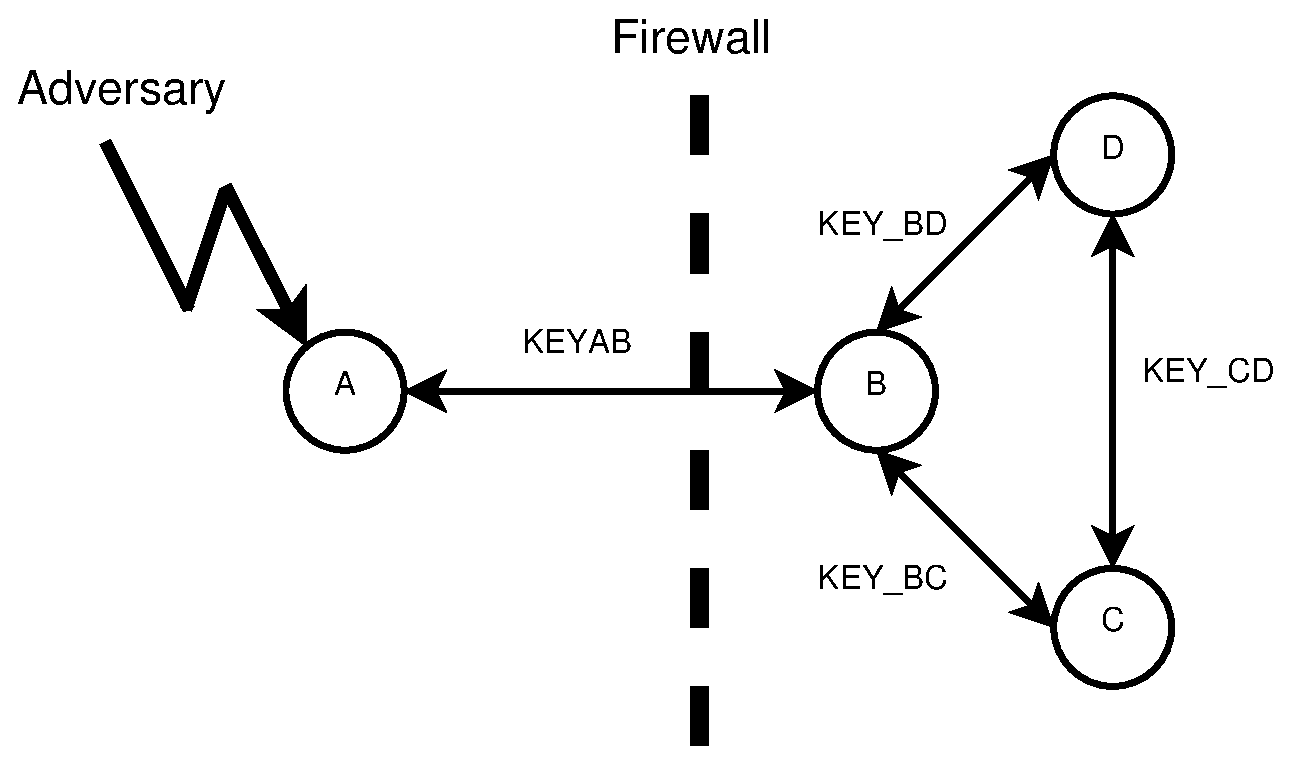
\includegraphics[width=0.8\textwidth]{figures/firewall2.eps}
% % Graphic for TeX using PGF
% Title: /home/hglanzer/ownCloud/Diplomarbeit/MasterThesisTemplate/figures/firewall.dia
% Creator: Dia v0.97.2
% CreationDate: Fri Dec  5 19:14:47 2014
% For: hglanzer
% \usepackage{tikz}
% The following commands are not supported in PSTricks at present
% We define them conditionally, so when they are implemented,
% this pgf file will use them.
\ifx\du\undefined
  \newlength{\du}
\fi
\setlength{\du}{15\unitlength}
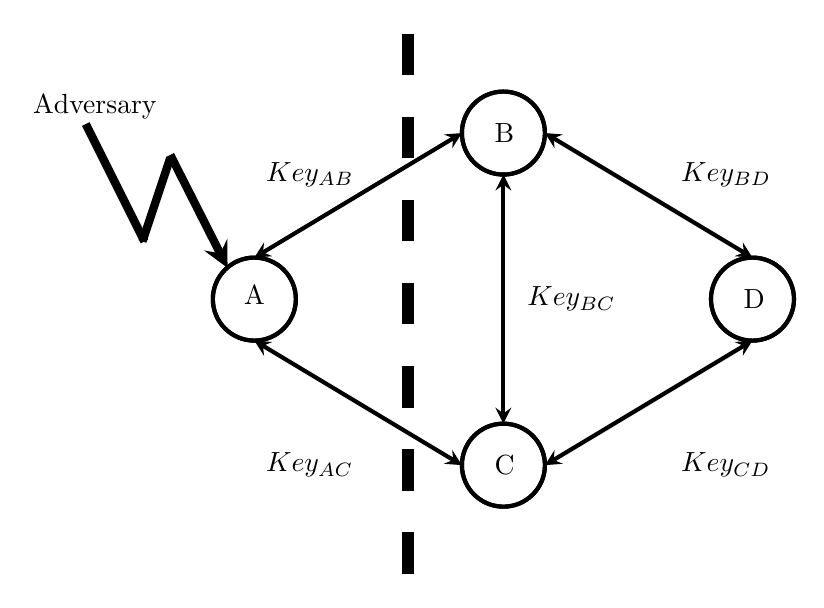
\begin{tikzpicture}
\pgftransformxscale{1.000000}
\pgftransformyscale{-1.000000}
\definecolor{dialinecolor}{rgb}{0.000000, 0.000000, 0.000000}
\pgfsetstrokecolor{dialinecolor}
\definecolor{dialinecolor}{rgb}{1.000000, 1.000000, 1.000000}
\pgfsetfillcolor{dialinecolor}
\pgfsetlinewidth{0.100000\du}
\pgfsetdash{}{0pt}
\pgfsetdash{}{0pt}
\pgfsetbuttcap
\pgfsetmiterjoin
\pgfsetlinewidth{0.100000\du}
\pgfsetbuttcap
\pgfsetmiterjoin
\pgfsetdash{}{0pt}
\definecolor{dialinecolor}{rgb}{1.000000, 1.000000, 1.000000}
\pgfsetfillcolor{dialinecolor}
\pgfpathellipse{\pgfpoint{12.000000\du}{5.000000\du}}{\pgfpoint{1.000000\du}{0\du}}{\pgfpoint{0\du}{1.000000\du}}
\pgfusepath{fill}
\definecolor{dialinecolor}{rgb}{0.000000, 0.000000, 0.000000}
\pgfsetstrokecolor{dialinecolor}
\pgfpathellipse{\pgfpoint{12.000000\du}{5.000000\du}}{\pgfpoint{1.000000\du}{0\du}}{\pgfpoint{0\du}{1.000000\du}}
\pgfusepath{stroke}
\pgfsetbuttcap
\pgfsetmiterjoin
\pgfsetdash{}{0pt}
\definecolor{dialinecolor}{rgb}{0.000000, 0.000000, 0.000000}
\pgfsetstrokecolor{dialinecolor}
\pgfpathellipse{\pgfpoint{12.000000\du}{5.000000\du}}{\pgfpoint{1.000000\du}{0\du}}{\pgfpoint{0\du}{1.000000\du}}
\pgfusepath{stroke}
\pgfsetlinewidth{0.100000\du}
\pgfsetdash{}{0pt}
\pgfsetdash{}{0pt}
\pgfsetbuttcap
\pgfsetmiterjoin
\pgfsetlinewidth{0.100000\du}
\pgfsetbuttcap
\pgfsetmiterjoin
\pgfsetdash{}{0pt}
\definecolor{dialinecolor}{rgb}{1.000000, 1.000000, 1.000000}
\pgfsetfillcolor{dialinecolor}
\pgfpathellipse{\pgfpoint{18.000000\du}{1.000000\du}}{\pgfpoint{1.000000\du}{0\du}}{\pgfpoint{0\du}{1.000000\du}}
\pgfusepath{fill}
\definecolor{dialinecolor}{rgb}{0.000000, 0.000000, 0.000000}
\pgfsetstrokecolor{dialinecolor}
\pgfpathellipse{\pgfpoint{18.000000\du}{1.000000\du}}{\pgfpoint{1.000000\du}{0\du}}{\pgfpoint{0\du}{1.000000\du}}
\pgfusepath{stroke}
\pgfsetbuttcap
\pgfsetmiterjoin
\pgfsetdash{}{0pt}
\definecolor{dialinecolor}{rgb}{0.000000, 0.000000, 0.000000}
\pgfsetstrokecolor{dialinecolor}
\pgfpathellipse{\pgfpoint{18.000000\du}{1.000000\du}}{\pgfpoint{1.000000\du}{0\du}}{\pgfpoint{0\du}{1.000000\du}}
\pgfusepath{stroke}
\pgfsetlinewidth{0.100000\du}
\pgfsetdash{}{0pt}
\pgfsetdash{}{0pt}
\pgfsetbuttcap
\pgfsetmiterjoin
\pgfsetlinewidth{0.100000\du}
\pgfsetbuttcap
\pgfsetmiterjoin
\pgfsetdash{}{0pt}
\definecolor{dialinecolor}{rgb}{1.000000, 1.000000, 1.000000}
\pgfsetfillcolor{dialinecolor}
\pgfpathellipse{\pgfpoint{18.000000\du}{9.000000\du}}{\pgfpoint{1.000000\du}{0\du}}{\pgfpoint{0\du}{1.000000\du}}
\pgfusepath{fill}
\definecolor{dialinecolor}{rgb}{0.000000, 0.000000, 0.000000}
\pgfsetstrokecolor{dialinecolor}
\pgfpathellipse{\pgfpoint{18.000000\du}{9.000000\du}}{\pgfpoint{1.000000\du}{0\du}}{\pgfpoint{0\du}{1.000000\du}}
\pgfusepath{stroke}
\pgfsetbuttcap
\pgfsetmiterjoin
\pgfsetdash{}{0pt}
\definecolor{dialinecolor}{rgb}{0.000000, 0.000000, 0.000000}
\pgfsetstrokecolor{dialinecolor}
\pgfpathellipse{\pgfpoint{18.000000\du}{9.000000\du}}{\pgfpoint{1.000000\du}{0\du}}{\pgfpoint{0\du}{1.000000\du}}
\pgfusepath{stroke}
\pgfsetlinewidth{0.100000\du}
\pgfsetdash{}{0pt}
\pgfsetdash{}{0pt}
\pgfsetbuttcap
\pgfsetmiterjoin
\pgfsetlinewidth{0.100000\du}
\pgfsetbuttcap
\pgfsetmiterjoin
\pgfsetdash{}{0pt}
\definecolor{dialinecolor}{rgb}{1.000000, 1.000000, 1.000000}
\pgfsetfillcolor{dialinecolor}
\pgfpathellipse{\pgfpoint{24.000000\du}{5.000000\du}}{\pgfpoint{1.000000\du}{0\du}}{\pgfpoint{0\du}{1.000000\du}}
\pgfusepath{fill}
\definecolor{dialinecolor}{rgb}{0.000000, 0.000000, 0.000000}
\pgfsetstrokecolor{dialinecolor}
\pgfpathellipse{\pgfpoint{24.000000\du}{5.000000\du}}{\pgfpoint{1.000000\du}{0\du}}{\pgfpoint{0\du}{1.000000\du}}
\pgfusepath{stroke}
\pgfsetbuttcap
\pgfsetmiterjoin
\pgfsetdash{}{0pt}
\definecolor{dialinecolor}{rgb}{0.000000, 0.000000, 0.000000}
\pgfsetstrokecolor{dialinecolor}
\pgfpathellipse{\pgfpoint{24.000000\du}{5.000000\du}}{\pgfpoint{1.000000\du}{0\du}}{\pgfpoint{0\du}{1.000000\du}}
\pgfusepath{stroke}
\pgfsetlinewidth{0.100000\du}
\pgfsetdash{}{0pt}
\pgfsetdash{}{0pt}
\pgfsetbuttcap
{
\definecolor{dialinecolor}{rgb}{0.000000, 0.000000, 0.000000}
\pgfsetfillcolor{dialinecolor}
% was here!!!
\pgfsetarrowsstart{stealth}
\pgfsetarrowsend{stealth}
\definecolor{dialinecolor}{rgb}{0.000000, 0.000000, 0.000000}
\pgfsetstrokecolor{dialinecolor}
\draw (17.000000\du,1.000000\du)--(12.000000\du,4.000000\du);
}
\pgfsetlinewidth{0.100000\du}
\pgfsetdash{}{0pt}
\pgfsetdash{}{0pt}
\pgfsetbuttcap
{
\definecolor{dialinecolor}{rgb}{0.000000, 0.000000, 0.000000}
\pgfsetfillcolor{dialinecolor}
% was here!!!
\pgfsetarrowsstart{stealth}
\pgfsetarrowsend{stealth}
\definecolor{dialinecolor}{rgb}{0.000000, 0.000000, 0.000000}
\pgfsetstrokecolor{dialinecolor}
\draw (12.000000\du,6.000000\du)--(17.000000\du,9.000000\du);
}
\pgfsetlinewidth{0.100000\du}
\pgfsetdash{}{0pt}
\pgfsetdash{}{0pt}
\pgfsetbuttcap
{
\definecolor{dialinecolor}{rgb}{0.000000, 0.000000, 0.000000}
\pgfsetfillcolor{dialinecolor}
% was here!!!
\pgfsetarrowsstart{stealth}
\pgfsetarrowsend{stealth}
\definecolor{dialinecolor}{rgb}{0.000000, 0.000000, 0.000000}
\pgfsetstrokecolor{dialinecolor}
\draw (19.000000\du,9.000000\du)--(24.000000\du,6.000000\du);
}
\pgfsetlinewidth{0.100000\du}
\pgfsetdash{}{0pt}
\pgfsetdash{}{0pt}
\pgfsetbuttcap
{
\definecolor{dialinecolor}{rgb}{0.000000, 0.000000, 0.000000}
\pgfsetfillcolor{dialinecolor}
% was here!!!
\pgfsetarrowsstart{stealth}
\pgfsetarrowsend{stealth}
\definecolor{dialinecolor}{rgb}{0.000000, 0.000000, 0.000000}
\pgfsetstrokecolor{dialinecolor}
\draw (19.000000\du,1.000000\du)--(24.000000\du,4.000000\du);
}
\pgfsetlinewidth{0.100000\du}
\pgfsetdash{}{0pt}
\pgfsetdash{}{0pt}
\pgfsetbuttcap
{
\definecolor{dialinecolor}{rgb}{0.000000, 0.000000, 0.000000}
\pgfsetfillcolor{dialinecolor}
% was here!!!
\pgfsetarrowsstart{stealth}
\pgfsetarrowsend{stealth}
\definecolor{dialinecolor}{rgb}{0.000000, 0.000000, 0.000000}
\pgfsetstrokecolor{dialinecolor}
\draw (18.000000\du,2.000000\du)--(18.000000\du,8.000000\du);
}
\pgfsetlinewidth{0.300000\du}
\pgfsetdash{{1.000000\du}{1.000000\du}}{0\du}
\pgfsetdash{{1.000000\du}{1.000000\du}}{0\du}
\pgfsetbuttcap
{
\definecolor{dialinecolor}{rgb}{0.000000, 0.000000, 0.000000}
\pgfsetfillcolor{dialinecolor}
% was here!!!
\definecolor{dialinecolor}{rgb}{0.000000, 0.000000, 0.000000}
\pgfsetstrokecolor{dialinecolor}
\draw (15.707107\du,-1.388909\du)--(15.707107\du,11.611091\du);
}
% setfont left to latex
\definecolor{dialinecolor}{rgb}{0.000000, 0.000000, 0.000000}
\pgfsetstrokecolor{dialinecolor}
\node[anchor=west] at (18.292893\du,5.000000\du){$Key_{BC}$};
% setfont left to latex
\definecolor{dialinecolor}{rgb}{0.000000, 0.000000, 0.000000}
\pgfsetstrokecolor{dialinecolor}
\node[anchor=west] at (11.469670\du,4.893934\du){A};
% setfont left to latex
\definecolor{dialinecolor}{rgb}{0.000000, 0.000000, 0.000000}
\pgfsetstrokecolor{dialinecolor}
\node[anchor=west] at (17.505025\du,1.000000\du){B};
% setfont left to latex
\definecolor{dialinecolor}{rgb}{0.000000, 0.000000, 0.000000}
\pgfsetstrokecolor{dialinecolor}
\node[anchor=west] at (17.505025\du,9.000000\du){C};
% setfont left to latex
\definecolor{dialinecolor}{rgb}{0.000000, 0.000000, 0.000000}
\pgfsetstrokecolor{dialinecolor}
\node[anchor=west] at (23.505025\du,5.000000\du){D};
% setfont left to latex
\definecolor{dialinecolor}{rgb}{0.000000, 0.000000, 0.000000}
\pgfsetstrokecolor{dialinecolor}
\node[anchor=west] at (12.000000\du,2.000000\du){$Key_{AB}$};
% setfont left to latex
\definecolor{dialinecolor}{rgb}{0.000000, 0.000000, 0.000000}
\pgfsetstrokecolor{dialinecolor}
\node[anchor=west] at (12.000000\du,9.000000\du){$Key_{AC}$};
% setfont left to latex
\definecolor{dialinecolor}{rgb}{0.000000, 0.000000, 0.000000}
\pgfsetstrokecolor{dialinecolor}
\node[anchor=west] at (22.000000\du,2.000000\du){$Key_{BD}$};
% setfont left to latex
\definecolor{dialinecolor}{rgb}{0.000000, 0.000000, 0.000000}
\pgfsetstrokecolor{dialinecolor}
\node[anchor=west] at (22.000000\du,9.000000\du){$Key_{CD}$};
% setfont left to latex
\definecolor{dialinecolor}{rgb}{0.000000, 0.000000, 0.000000}
\pgfsetstrokecolor{dialinecolor}
\node[anchor=west] at (14.000000\du,9.000000\du){};
\pgfsetlinewidth{0.200000\du}
\pgfsetdash{}{0pt}
\pgfsetdash{}{0pt}
\pgfsetbuttcap
{
\definecolor{dialinecolor}{rgb}{0.000000, 0.000000, 0.000000}
\pgfsetfillcolor{dialinecolor}
% was here!!!
\definecolor{dialinecolor}{rgb}{0.000000, 0.000000, 0.000000}
\pgfsetstrokecolor{dialinecolor}
\draw (7.939094\du,0.782827\du)--(9.353307\du,3.611255\du);
}
\pgfsetlinewidth{0.200000\du}
\pgfsetdash{}{0pt}
\pgfsetdash{}{0pt}
\pgfsetbuttcap
{
\definecolor{dialinecolor}{rgb}{0.000000, 0.000000, 0.000000}
\pgfsetfillcolor{dialinecolor}
% was here!!!
\definecolor{dialinecolor}{rgb}{0.000000, 0.000000, 0.000000}
\pgfsetstrokecolor{dialinecolor}
\draw (9.303307\du,3.611255\du)--(9.975059\du,1.596000\du);
}
\pgfsetlinewidth{0.200000\du}
\pgfsetdash{}{0pt}
\pgfsetdash{}{0pt}
\pgfsetbuttcap
{
\definecolor{dialinecolor}{rgb}{0.000000, 0.000000, 0.000000}
\pgfsetfillcolor{dialinecolor}
% was here!!!
\pgfsetarrowsend{stealth}
\definecolor{dialinecolor}{rgb}{0.000000, 0.000000, 0.000000}
\pgfsetstrokecolor{dialinecolor}
\draw (9.975059\du,1.525290\du)--(11.353917\du,4.247651\du);
}
% setfont left to latex
\definecolor{dialinecolor}{rgb}{0.000000, 0.000000, 0.000000}
\pgfsetstrokecolor{dialinecolor}
\node[anchor=west] at (6.439525\du,0.358563\du){Adversary};
\end{tikzpicture}

 \caption{Firewall}
 \label{fig:firewall}
\end{figure}
As stated above, to be able to use different keys every security gateway has to know how to reach a given address so that the data can be encrypted
exclusively for the responsible gateway. The solution to this problem is to maintain some kind of routing table, mapping group and individual addresses of unsecured
\gls{knx} devices to individual addresses of responsible security gateways	.
Such a routing table can be built statically at setup time, with the obvious disadvantage
that the exact topology of the to be applied network has to be known in advance, thus reducing the flexibility. Here, every security gateway holds a static 
table which consists of mappings between individual- or group addresses of unsecured \gls{knx} devices and individual addresses of security gateways at the border
between the secured and the unsecured \gls{knx} network, as well as all keys used for the particular security level the gateway belongs to.
This table would be generated once, after the topology of the network has been fixed, and must be equipped with the proper keys and can then
be copied to the security gateways constituting the secured \gls{knx} area. New security gateways can be deployed as long as they only introduce sending 
unsecured \gls{knx} devices, whose recipients are already mapped, known group addresses. A new group address, introduced by a newly installed device behind
an already existing security gateway, will not be reachable, simply because the routing information is not available. 
Another disadvantage is that the deployment of new
security gateways, connecting devices with new or already known group addresses, is impossible as the individual address of the new gateway - which of
course must be unique - is unknown to the existing setup, thus making the new unsecured \gls{knx} devices unreachable.
\\
To tackle this problem, another approach would be to build this mapping table dynamically. Therefore, every security gateway must periodically poll
on it's unsecured lines for \gls{knx} devices, thus populating a list of reachable \gls{knx} devices. Whenever a 
device wants to send data to a group address, it has to do a lookup first to obtain the individual addresses of the responsible security gateways: the lookup
must contain the wanted group address, as well as the senders public key.
Every 
gateway which finds the wanted group address in its group list must reply with an according message to the requester, thus announcing that it is responsible
for delivering data to the wanted group address, and must also publish it's own public key, thus allowing pairwise end-to-end encryption.
This procedure requires no a priori knowledge of
the network topology, so security gateways can be added to the network as well as unsecured \gls{knx} devices behind new or existing gateways at any time. This
flexibility of course has to be purchased with increased complexity as well as additional traffic introduced into the network.
\\
\\
A middle course is chosen: the reachable group address list is generated whenever a new security gateway is added to the network,
 handling discovery of this group addresses as described
above. This allows to deploy new security gateways with connected unsecured devices, thus achieving a comprise between flexibility and complexity. 
\\
Sending data to a group address therefor follows the triad discovery request, discovery response and actual data transfer, shown in figure \ref{fig:prot1}. Broadcast
messages are depicted as solid end of the arrow, the rest denoting unicast messages.
\begin{figure}
  \centering
    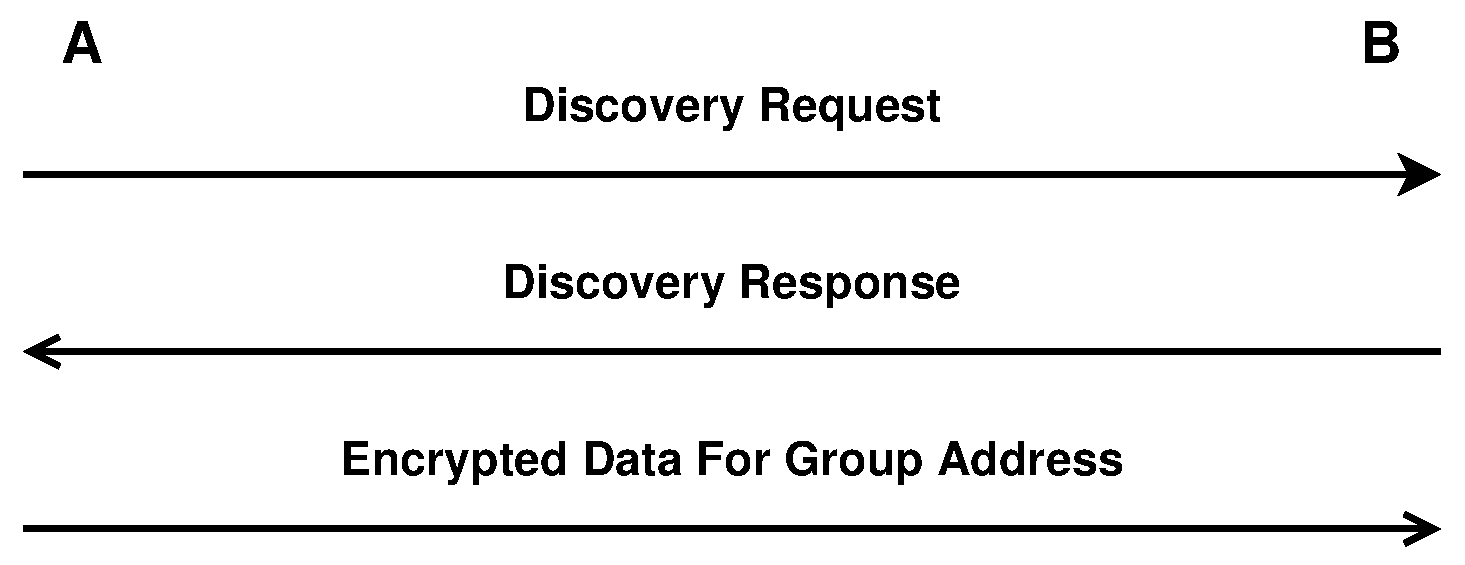
\includegraphics[width=0.8\textwidth]{figures/protokoll1.eps}
 \caption{Communication schema}
 \label{fig:prot1}
\end{figure}
To enable multiple devices to announce responsibility for a group address, the device wanting to transmit data to this group address must accept discovery responses
following it's request message for a short time window.
\\
\\
The discovery messages generated by security gateways should be encrypted too. Although these datagrams don't contain \gls{knx} data per se, they allow
a listening adversary to learn the topology of the network, knowledge which can be valuable for developing an attack strategy, as well as generating meta data.
For example, if an attacker learns that a particular security gateway is responsible for only one group address and further gets knowledge that this 
group address is responsible for switching a light (i.e. by visual observation), the attacker afterwards may be able to derive a personal profile just by seeing
packages for this group address, although the payload of the datagrams to the responsible security gateway are encrypted.
If the discovery messages are encrypted too the adversary doesn't know how many and what
group addresses are behind a specif gateway, and it will be harder to derive personal profiles or to gather knowledge of the network topology.
\\
Discovery request messages must be broadcast messages, readable by all security gateways. To limit the protocol overhead, a global network key is used here.
\\
\\
To provide authenticity, all datagrams passing the secured \gls{knx} network must contain a \gls{mac2} to prevent modification of them.
\\
Defense against replay attacks is achieved by counters.These must be strictly monotonically
increasing and must not overflow. The counters can be compared to an initialization vector that prevents the mapping of same cleartext messages to same ciphertext messages
under the same encryption key.
\\
Two different types of counters are used: one global counter $Ctr_{global}$, used for avoiding replay attacks against discovery messages. A second kind of counter
is used for the actual data transfer. Beside avoiding replay attacks, this counter is necessary to detect and delete duplicates, caused by the redundant network, 
see \ref{ctrAvail} for details.
\\
Usage of the global counter $Ctr_{global}$ raises another question, namely how a new device gets knowledge of the actual value of $Ctr_{global}$.
Therefor, a sync service must be defined, allowing a newly powered up device to synchronize with the rest of the network \ref{fig:syncProt}.
\begin{figure}
  \centering
    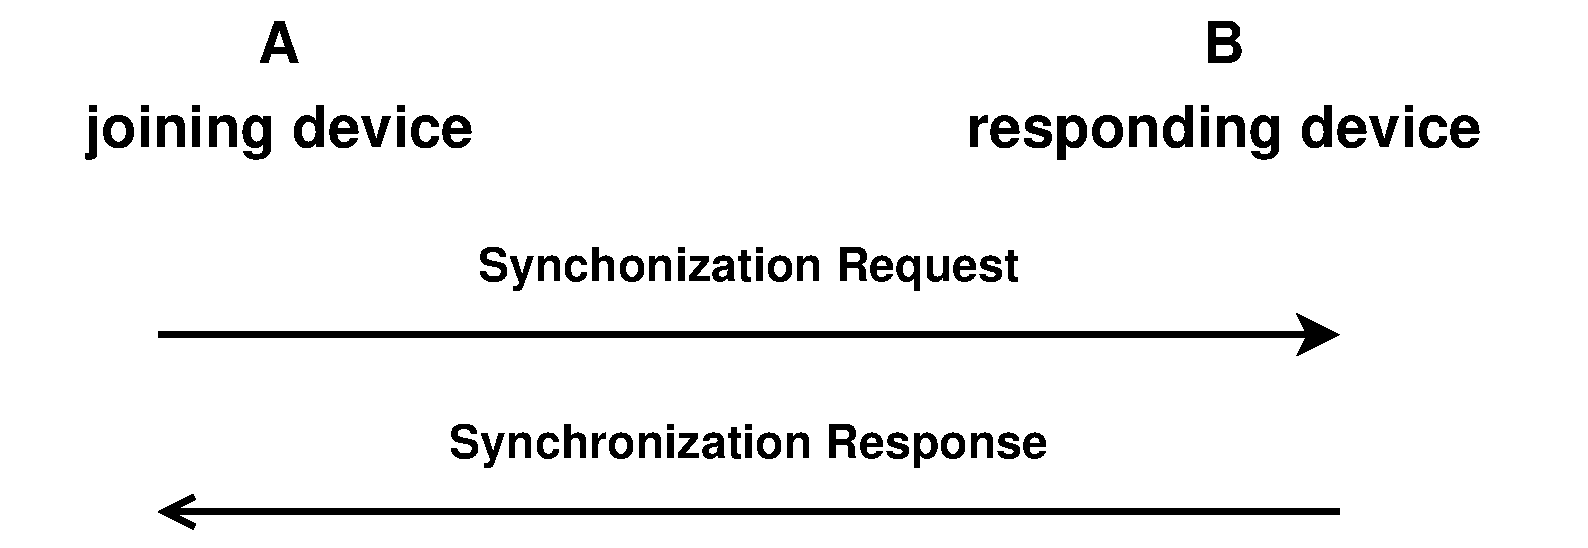
\includegraphics[width=0.8\textwidth]{figures/protSync.eps}
 \caption{Synchronization serice}
 \label{fig:syncProt}
\end{figure}
Replay attacks are mitigated by including the actual time into \gls{mac2} calculation. Low temporal resolution relaxes time-synchronization issues between
different devices.

\subsubsection{Key Management}

While it would be possible to use a centralized concept, no trusted on-line party is used in this work. A centralized approach would need fall-back key servers
which inherit the task of generating and distributing keys and parameters in case of a master key server failure. Otherwise, the network would suffer from a
single point of failure in case no such fall-back mechanism is applied, an assumption that would clearly disqualify the design as highly available.
\\
The following keys are used:

\begin{itemize}
 \item A long-term key known to all security gateways is used. As already stated, this key must be copied to every device at setup time. 
This pre-shared key $k_{psk}$ is used for symmetric encryption and serves different purposes: first, it is used to authenticate synchronization messages.
Secondly, this key $k_{psk}$ is used to encrypt discovery requests and discovery responses.
 %\item $k_{global}$ is used to authenticate and encrypt locally generated and decrypt received discovery requests, as well as to authenticate and encrypt
 %locally generated discovery responses and decrypt received ones. These discovery service datagrams securely transport the third type of keys:
 \item Asymmetric keys are used for end-to-end encryption of the actual data packages between 2 security gateways. \gls{ecdh} serves as key negotiation algorithm.
 To protect against man-in-the-middle attacks, authenticity of the \gls{dh} parameters must be assured.
 \item This is the task of the third kind of keys: another pre-shared key is used to authenticate the \gls{dh} parameters.
\end{itemize}


\subsection{Redundancy Related Architectural Overview}\label{ctrAvail}
 
Whenever a \gls{knx} package is
generated by a device on an unsecured line (called client), the connected security gateway will read, duplicate and encapsulate it into another \gls{knx} frame 
and then send over booth lines. If booth lines are available, i.e. there is, for example, no shortcut, a receiving security gateway will receive 2
different \gls{knx} frames encapsulating the same
payload, which itself is the \gls{knx} frame generated by the \gls{knx} client device in the first place. 
One message must be discarded to avoid duplicates. 
This is achieved with a monotonically increasing counter that also guards against replay attacks: whenever a package, generated by a client, enters the
network, a counter for outgoing packages is incremented. 
This counter must be unambiguously referenced by the source address of the origin cleartext message. 
The receiving side must maintain a counter for incoming packets, 
also uniquely identified by a source address. If booth lines are available, one message will be handled first and trigger an incrementation of the
corresponding source address counter. The duplicated message, which is handled after that, can safely be discarded because the corresponding counter
value will be less than the saved value.
% Nevertheless which package from which secure line is forwarded to the unsecured line, each line must acknowledge
% every received package: this is done by generating a special acknowledge frame which is sent back to the sending gateway. The payload of this package must
% allow the sending gateway to unambiguously identify the acknowledged package, i.e. it must bear source and destination address of the package generated
% by the client, as well as the used counter value. As a consequence, these acknowledgement frames must be encrypted and authenticated as well.
% If no acknowledgement frame is received within time $t_{ACK}$, a retransmission is done on booth lines. This retransmission simply re-submits the same
% package with the same counter value again. Regarding the security this is no problem because a passive attacker can not learn anything from such a repeated
% package.


\subsection{Operational Constraints}

The introduction of encapsulating security gateways implicates that some timing constraints, defined by \gls{knx}, cannot be met:

\begin{itemize}
 \item Acknowledge frames, as defined in \gls{knx} and introduced in chapter \ref{ch:knx}, cannot be guaranteed to be delivered within the specified deadlines: whenever
 a new \gls{knx} datagram is generated by a client, at first the discovery phase has to occur. Only after that the to-acknowledged frame is sent. So there are
 multiple delays introduced, stalling the delivery: the first delay is caused by sending of the discovery package.
 After that, a second delay occurs because the security gateway must wait for the discovery response(s), possibly retransmitting the discovery request
 in case of a timeout. After receiving discovery responses, the third delay is caused by sending the actual, encapsulated
 client package to the responsible security gateway(s), which then must check the datagram, unpack it and forward it on it's unsecured line.
 Only after that, all addressed, unsecured clients would be able to acknowledge the received frames
 to their local security gateways,
 which must forwarded the acknowledgement frame to the origin security gateway, causing another delay. Finally, the acknowledgement frame must be forwarded to the sender of
 the origin data frame, causing another delay.
 These delays will always occur, and most of them cannot be restricted, thus destroying the tight timing constraints for acknowledgement frames, as defined
 by the \gls{knx} standard. This
 will most likely result in multiple retransmissions of the same \gls{knx} packages
 by the client because the client's timer will generate a timeout. The only way to solve this is to immediately acknowledge a client frame by the security
 gateway that it is connected to. On the receiving side, the client will generate an acknowledge
 frame, which must be discarded by it's security gateway.
 \item Similar arguments avoid the processing of Poll-Data Frames. Here, event more stringent timing constraints are to be met, see chapter \ref{ch:knx}. 
\end{itemize}

\section{Services}

Except from the data service, handling the actual data transfer of the \gls{knx} payloads, 2 additional services are necessary, following the assumptions above.
These two services, handling synchronization and discovery, are defined as following and are summarized as management services.

\begin{center}
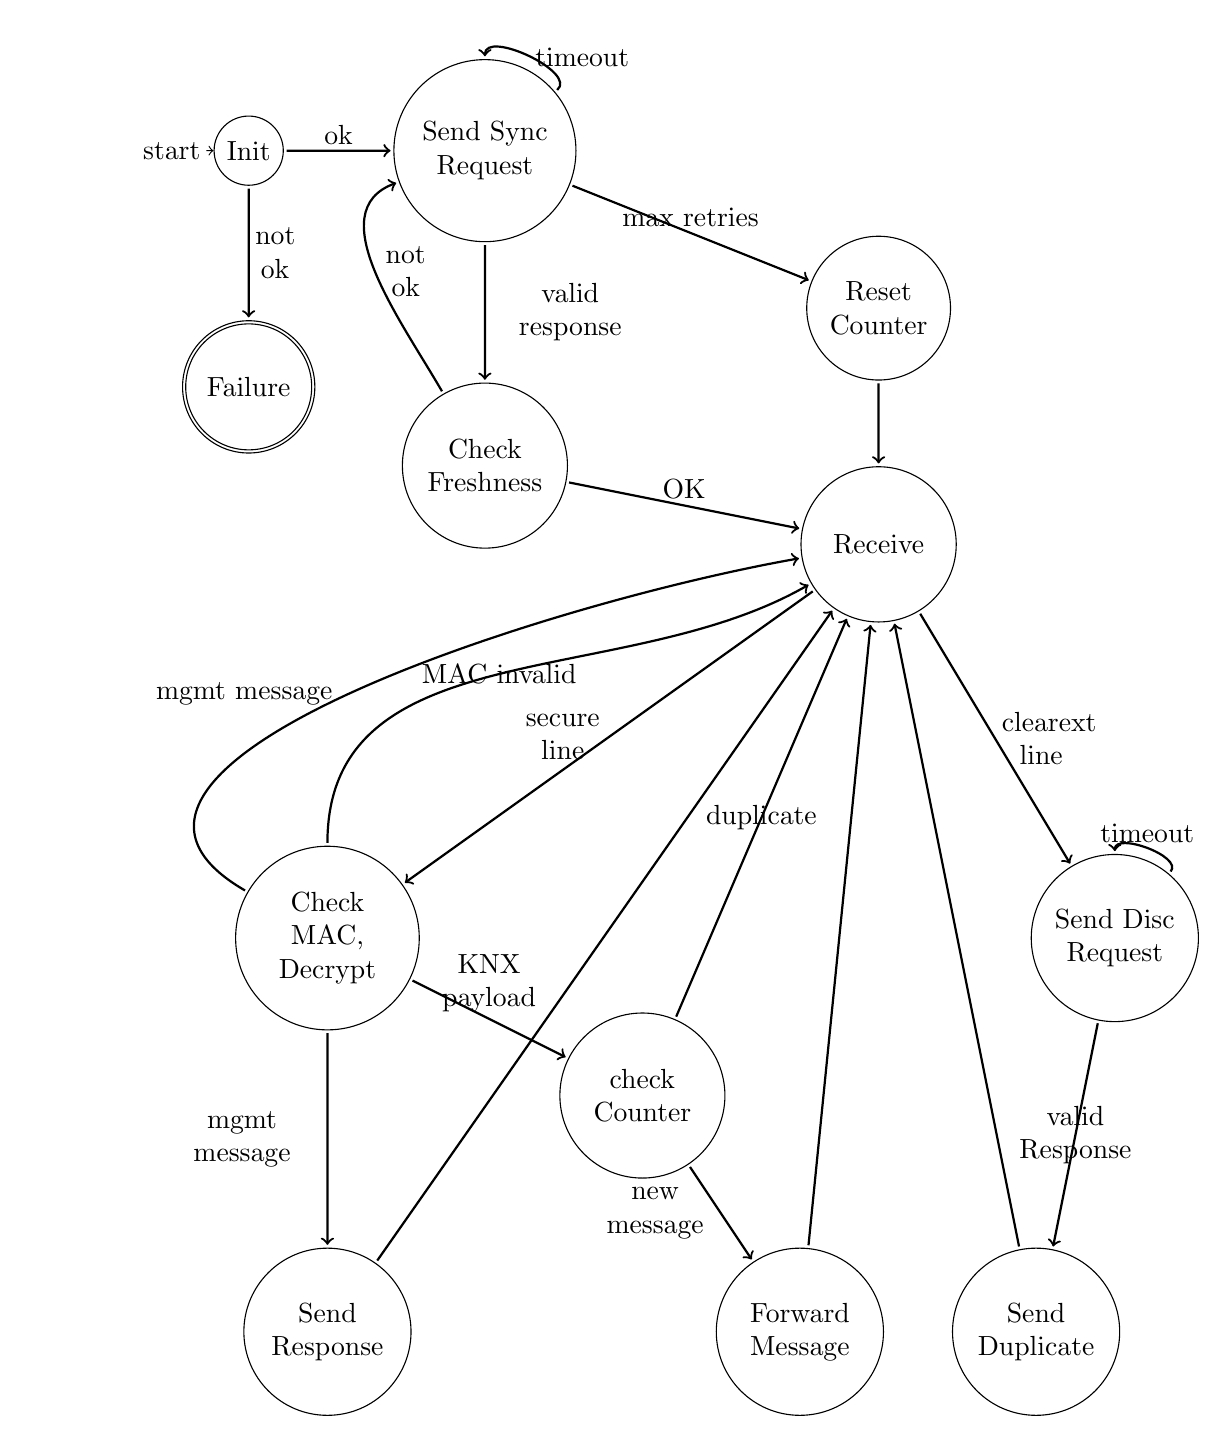
\begin{tikzpicture}[scale=0.2]
\tikzstyle{every node}+=[inner sep=2pt]
\tikzstyle{arrow}=[draw, -latex] 
\tikzset{
    pil/.style={
           ->,
           thick,
           shorten <=1pt,
           shorten >=1pt,}
}

\usetikzlibrary{automata,positioning}
\usetikzlibrary{positioning}

\node[state,initial]												at (45,35)			(init)		{Init}; 
\node[state, text width=2cm,align=center] 	at (60,35)		(sync)	{Send Sync Request};
\node[state, text width=1.5cm,align=center] 	at (45,20)	(fail)	{Failure}; 
\draw [black]	(45,20) circle (4);
\node[state, text width=1.5cm,align=center] 	at (85,25)		(res)	{Reset Counter};
\node[state, text width=1.8cm,align=center] 	at (60,15)		(chkFresh)	{Check Freshness};
\node[state, text width=1.8cm,align=center] 	at (85,10)		(rcv)	{Receive};
\node[state, text width=1.8cm,align=center] 	at (50,-15)		(chkMAC)	{Check MAC, Decrypt};
\node[state, text width=1.8cm,align=center] 	at (100,-15)		(discReq)	{Send Disc Request};

\node[state, text width=1.8cm,align=center] 	at (50,-40)		(sendResp)	{Send Response};
\node[state, text width=1.8cm,align=center] 	at (70,-25)		(chkDup)	{check Counter};
\node[state, text width=1.8cm,align=center] 	at (80,-40)		(fwd)	{Forward Message};

\node[state, text width=1.8cm,align=center] 	at (95,-40)		(sendDup)	{Send Duplicate};


\path[pil,->] (init)  edge[above] node[text width=1cm,align=center] {ok} (sync); 
\path[pil,->] (init)  edge[right] node[text width=0.5cm,align=center] {not ok} (fail); 
\path[pil,->] (sync)  edge[right,out=40,in=90] node[text width=1cm,align=center] {timeout} (sync); 
\path[pil,->] (sync)  edge[above] node[text width=2cm,align=center] {max retries} (res); 
\path[pil,->] (sync)  edge[right] node[text width=2cm,align=center] {valid response} (chkFresh); 
\path[pil,->] (chkFresh)  edge[right,out=120, in=200] node[text width=0.6cm,align=center] {not ok} (sync); 
\path[pil,->] (res)  edge[above] node[text width=2cm,align=center] {} (rcv); 
\path[pil,->] (chkFresh)  edge[above] node[text width=2cm,align=center] {OK} (rcv); 
\path[pil,->] (rcv)  edge[left] node[text width=1cm,align=center] {secure line} (chkMAC); 
\path[pil,->] (chkMAC)  edge[out=90,in=210] node[text width=2cm,align=center] {MAC invalid} (rcv); 
\path[pil,->] (rcv)  edge[right] node[text width=1cm,align=center] {clearext line} (discReq); 
\path[pil,->] (discReq)  edge[above,out=50,in=90] node[text width=1.2cm,align=center] {timeout} (discReq);
\path[pil,->] (discReq)  edge[] node[text width=2cm,align=center] {valid Response} (sendDup); 

\path[pil,->] (chkMAC)  edge[left] node[text width=2cm,align=center] {mgmt message} (sendResp); 
\path[pil,->] (chkMAC)  edge[left,out=150,in=190] node[text width=2.5cm,align=center] {mgmt message} (rcv); 
\path[pil,->] (sendResp)  edge[left] node[text width=2.5cm,align=center] {} (rcv); 
\path[pil,->] (fwd)  edge[left] node[text width=1cm,align=center] {} (rcv); 
\path[pil,->] (chkMAC)  edge[above] node[text width=1.4cm,align=center] {KNX payload} (chkDup); 
\path[pil,->] (chkDup)  edge[] node[text width=1.5cm,align=center] {duplicate} (rcv); 
\path[pil,->] (chkDup)  edge[left] node[text width=1.5cm,align=center] {new message} (fwd); 
\path[pil,->] (sendDup)  edge[] node[text width=2cm,align=left] {} (rcv); 

\end{tikzpicture}
\end{center}

\subsection{Synchronization service}

As stated, a new gateway, joining the network, must get knowledge of the actual value of $Ctr_{global}$. This is achieved by sending a broadcast message, 
serving as synchronization request, containing the device's local time in seconds, and the header flags in the secure header set accordingly, determining
the frame as synchronization request \ref{fig:syncReqFormat}.
\begin{figure}
  \centering
    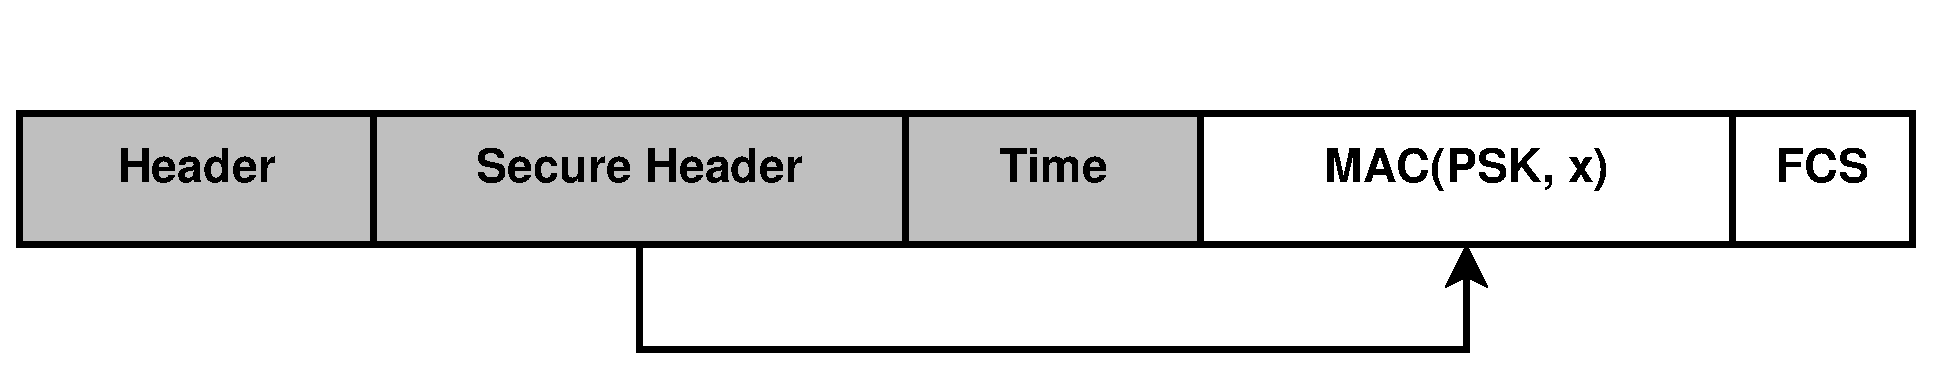
\includegraphics[width=1\textwidth]{figures/formatSyncReq.eps}
 \caption{Synchronization request package layout}
 \label{fig:syncReqFormat}
\end{figure}
\\
\\
Every device receiving such a request checks the integrity of the message first by recalculating the \gls{mac2}. Afterwards, freshness is checked by comparing
the supplied time with it's local time. If the timing information equals the device's own local time, the device sends a synchronization response
frame, containing it's local time and the actual counter value \ref{fig:syncResFormat}. The accuracy of the time comparison is deliberately reduced by defining
a window of allowed deviation. This allows a new device to join the network even it's local time and the local time of the answering device are not 
perfectly synchronized.
\\


\begin{figure}
  \centering
    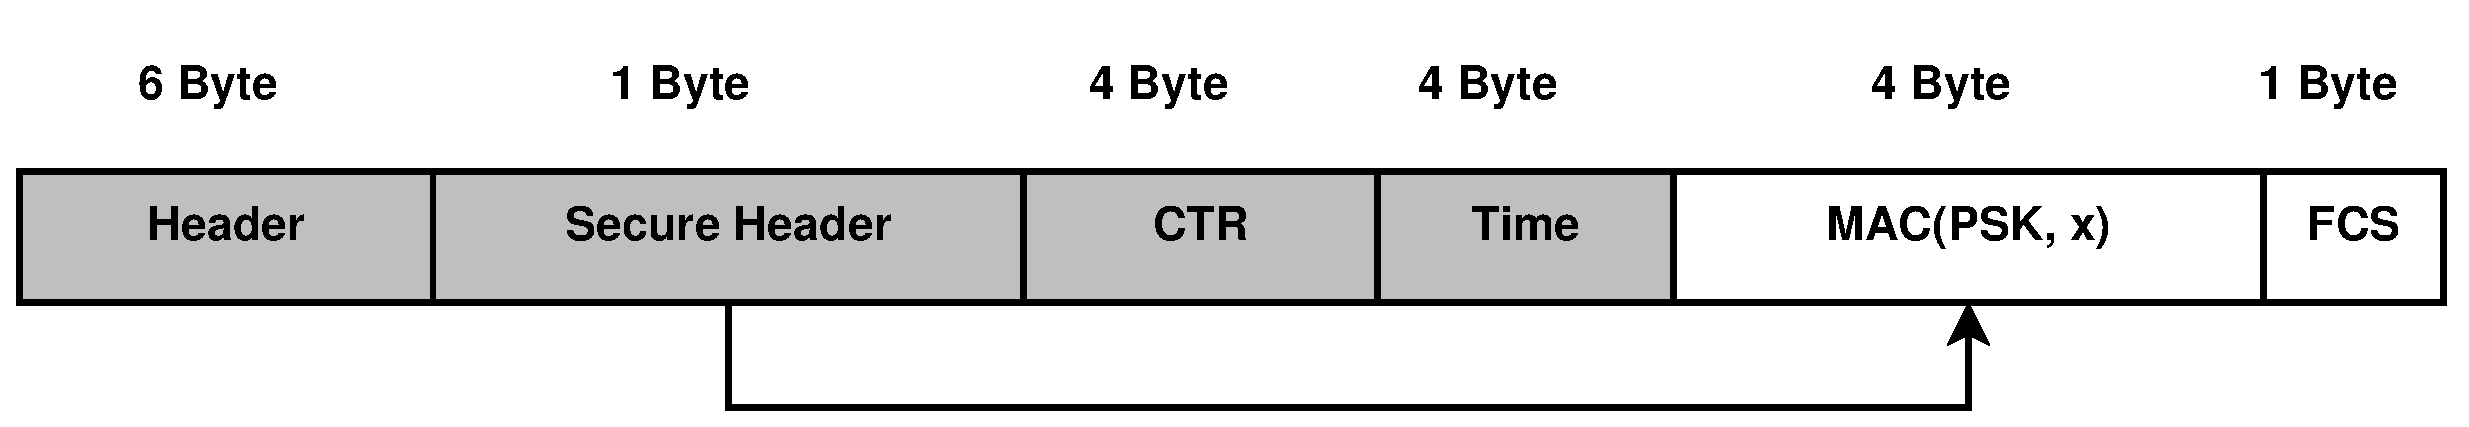
\includegraphics[width=1\textwidth]{figures/formatSyncRes.eps}
 \caption{Synchronization response package layout}
 \label{fig:syncResFormat}
\end{figure}
To allow a device to synchronize despite poor local clock synchronization,  
\subsection{Discovery service}

\subsection{Data service}
